\documentclass{beamer}
\usepackage{etex}

% Thematics
\PassOptionsToPackage{subsection=false}{beamerouterthememiniframes}
\usetheme{Szeged}
\usecolortheme{beaver}
\setbeamercolor{block title}{fg=darkred}
\setbeamercolor{item}{fg=darkred}
\setbeamertemplate{navigation symbols}{}
\let\oldsection\section
\renewcommand{\section}[1]{\oldsection{\textsc{#1}}\subsection{}}

% Graphics
\usepackage{graphicx}
\usepackage{tikz}
%\usetikzlibrary{arrows}
\usepackage[pdf]{pstricks}
\psset{unit=0.9in,linewidth=0.02,arrows=C-C,arrowsize=0.2}
\newcommand{\pscophylogeny}{
\begin{pspicture}(18,12)
\psset{unit=0.2cm,linewidth=0.2,arrowsize=0.2}
\psline[linecolor=blue](0,0)(10,10)
\psline[linecolor=blue](4,0)(2,2)
\psline[linecolor=blue](8,0)(4,4)
\psline[linecolor=blue](12,0)(14,2)
\psline[linecolor=blue](16,0)(8,8)
\psline[linecolor=red](1,0)(11,10)
\psline[linecolor=red,arrows=-o](17,0)(9,8)
\psline[linecolor=red,arrows=-o](13,0)(15,2)
\psline[linecolor=red](7,3)(14,3)
\psline[linecolor=red,arrows=<-](10,3)(14,3)
\psline[linecolor=red](10,0)(7,3)
\psline[linecolor=red,arrows=-o](9,0)(5,4)
\psline[linecolor=red,arrows=-o](4,1)(3,2)
\rput{135}(4,1){\LARGE\textcolor{red}{\textsf{\textbf{x}}}}
\psline[linecolor=red](18,0)(17,1)
\psline[linecolor=red,arrows=*-](16,1)(17,1)
\end{pspicture}
}
%\usepackage{pgfplots}

% Maths
\usepackage{amsmath}
\usepackage{mathtools}
\usepackage{commath}
\newcommand{\R}{\ensuremath{\mathcal{R}}}

%\makeatother

\usepackage{hanging}

\newcommand\blfootnote[1]{
  \begingroup
  \renewcommand\thefootnote{}\footnote{#1}
  \addtocounter{footnote}{-1}
  \endgroup
}

% Title page
\title[Bayesian Reconstruction of Coevolutionary Histories]{Bayesian Reconstruction of \\ Coevolutionary Histories}
\author{Arman Bilge\vspace{-0.15in}}
\institute[Arman Bilge]{\vspace{-0.25in}}%\\Faculty of Science\\The University of Auckland}
\date{\vspace{-0.25in}\\March 13, 2013}
\titlegraphic{
\begin{pspicture}(18,12)
\psset{unit=0.3cm,linewidth=0.2,arrowsize=1}
\psline[linecolor=blue](0,0)(10,10)
\psline[linecolor=blue](4,0)(2,2)
\psline[linecolor=blue](8,0)(4,4)
\psline[linecolor=blue](12,0)(14,2)
\psline[linecolor=blue](16,0)(8,8)
\psline[linecolor=red](1,0)(11,10)
\psline[linecolor=red,arrows=-o](17,0)(9,8)
\psline[linecolor=red,arrows=-o](13,0)(15,2)
\psline[linecolor=red](7,3)(14,3)
\psline[linecolor=red,arrows=<-](10,3)(14,3)
\psline[linecolor=red](10,0)(7,3)
\psline[linecolor=red,arrows=-o](9,0)(5,4)
\psline[linecolor=red,arrows=-o](4,1)(3,2)
\rput{135}(4,1){\LARGE\textcolor{red}{\textsf{\textbf{x}}}}
\psline[linecolor=red](18,0)(17,1)
\psline[linecolor=red,arrows=*-](16,1)(17,1)
\end{pspicture}
}

\begin{document}

%\begin{frame}{tikz}
%
%\begin{tikzpicture}[x=0.3cm, y=0.3cm, line width=0.06cm, arrowhead=0.03cm]
%
%\draw [blue] (0,0) -- (10,10);
%\draw [blue] (4,0) -- (2,2);
%\draw [blue] (8,0) -- (4,4);
%\draw [blue] (12,0) -- (14,2);
%\draw [blue] (16,0) -- (8,8);
%\draw [red] (1,0) -- (11,10);
%\draw [red,-o] (17,0) -- (9,8);
%\draw [red,-o] (13,0) -- (15,2);
%\draw [red] (7,3) -- (14,3);
%\draw [red,stealth-] (10,3) -- (14,3);
%\draw [red,-o] (10,0) -- (7,3);
%\draw [red,-o] (9,0) -- (5,4);
%\draw [red] (4,1) -- (3,2);
%\draw [red] (18,0) -- (17,1);
%\draw [red,*-] (16,1) -- (17,1);
%
%\end{tikzpicture}
%
%\end{frame}

\frame{\titlepage}

\section{Introduction}

%\begin{frame}{Symbiotic Interactions are Fundamental to Life}
%
%\begin{columns}
%
%\begin{column}{0.556\textwidth}
%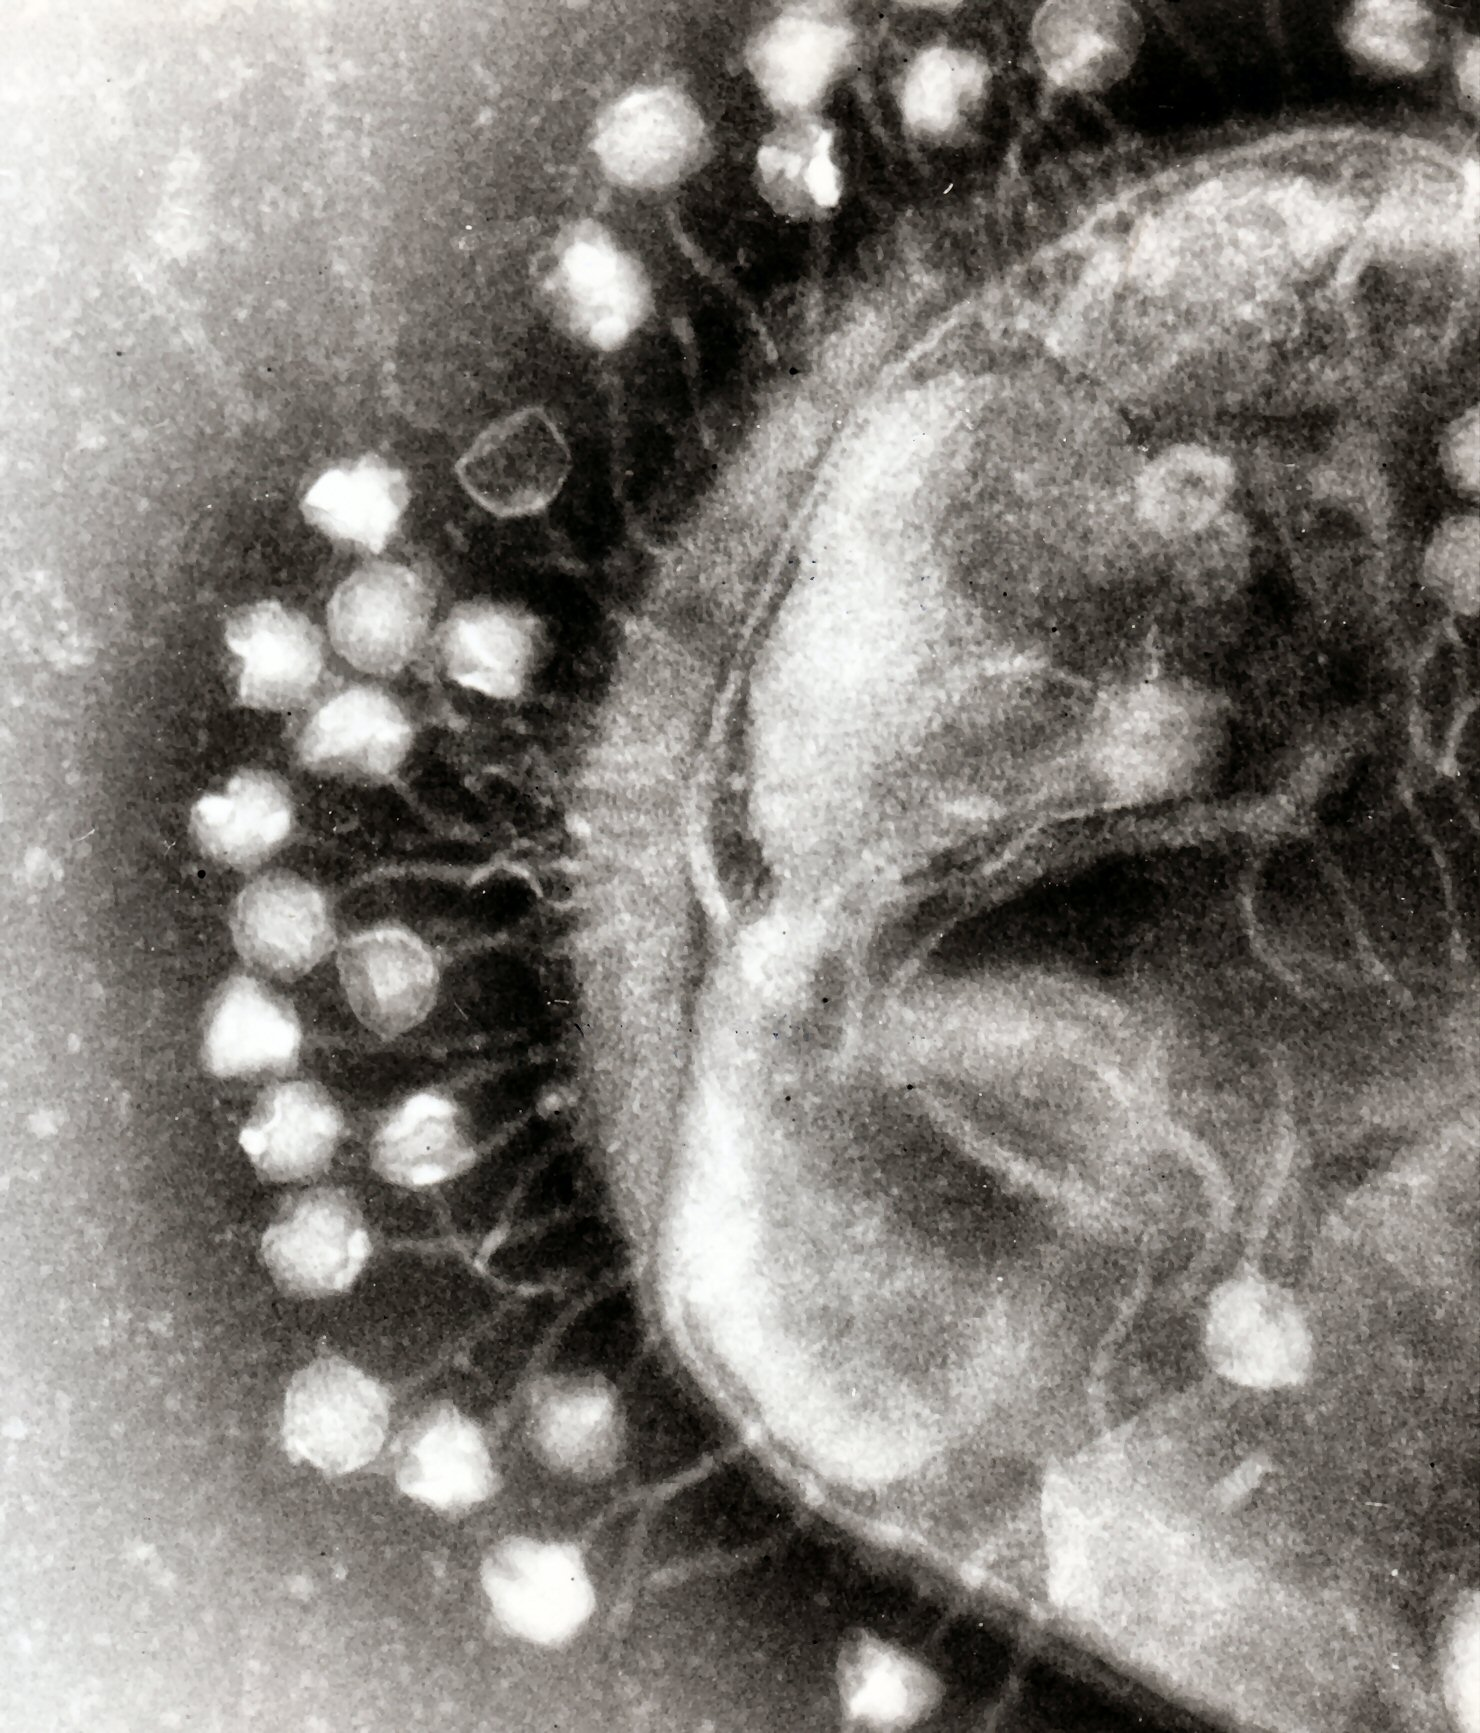
\includegraphics[width=\textwidth]{figures/symbioses/Phage.jpg}
%\end{column}
%
%\begin{column}{0.444\textwidth}
%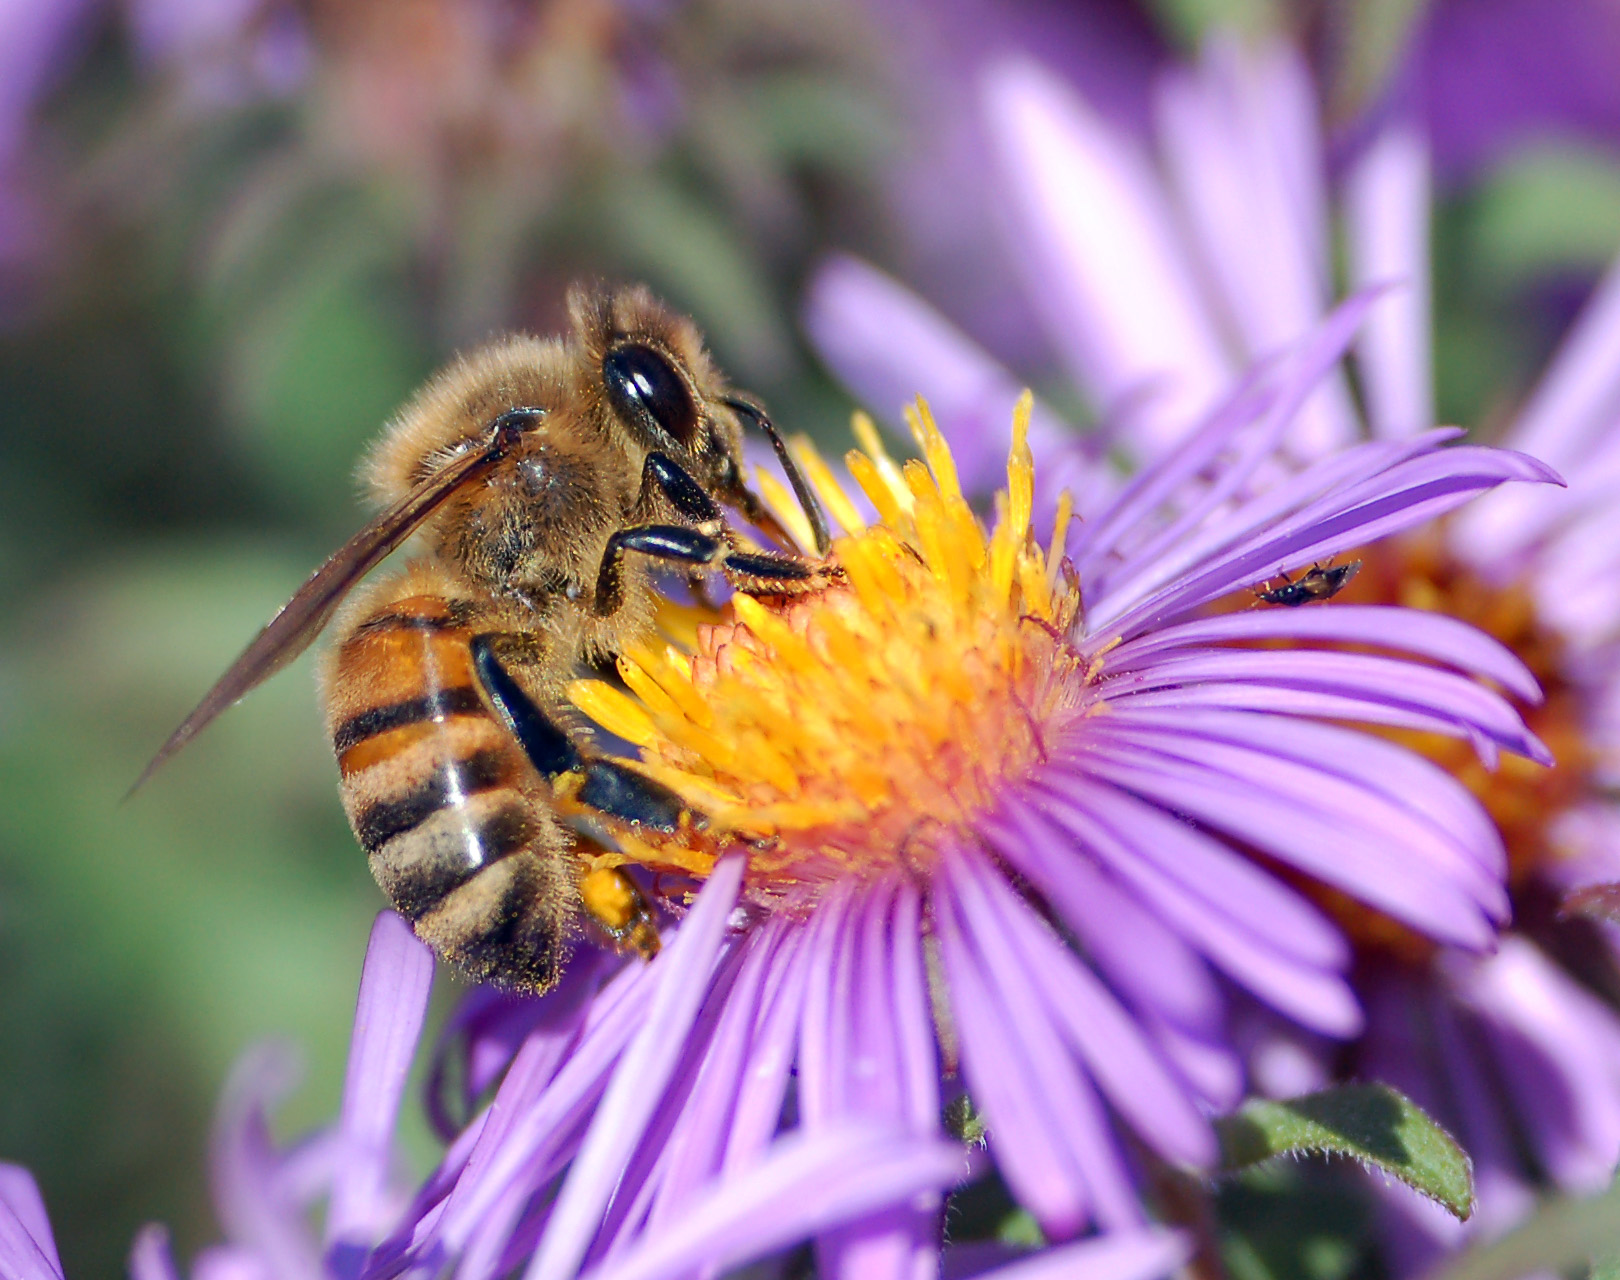
\includegraphics[width=\textwidth]{figures/symbioses/European_honey_bee_extracts_nectar.jpg}
%\vfil
%\includegraphics[width=\textwidth]{figures/symbioses/Clown_fish_in_the_Andaman_Coral_Reef.jpg}
%\end{column}
%
%\end{columns}
%
%\end{frame}

\begin{frame}{Phylogenetic Evidence for Cycad--Weevil Coevolution}

\centering

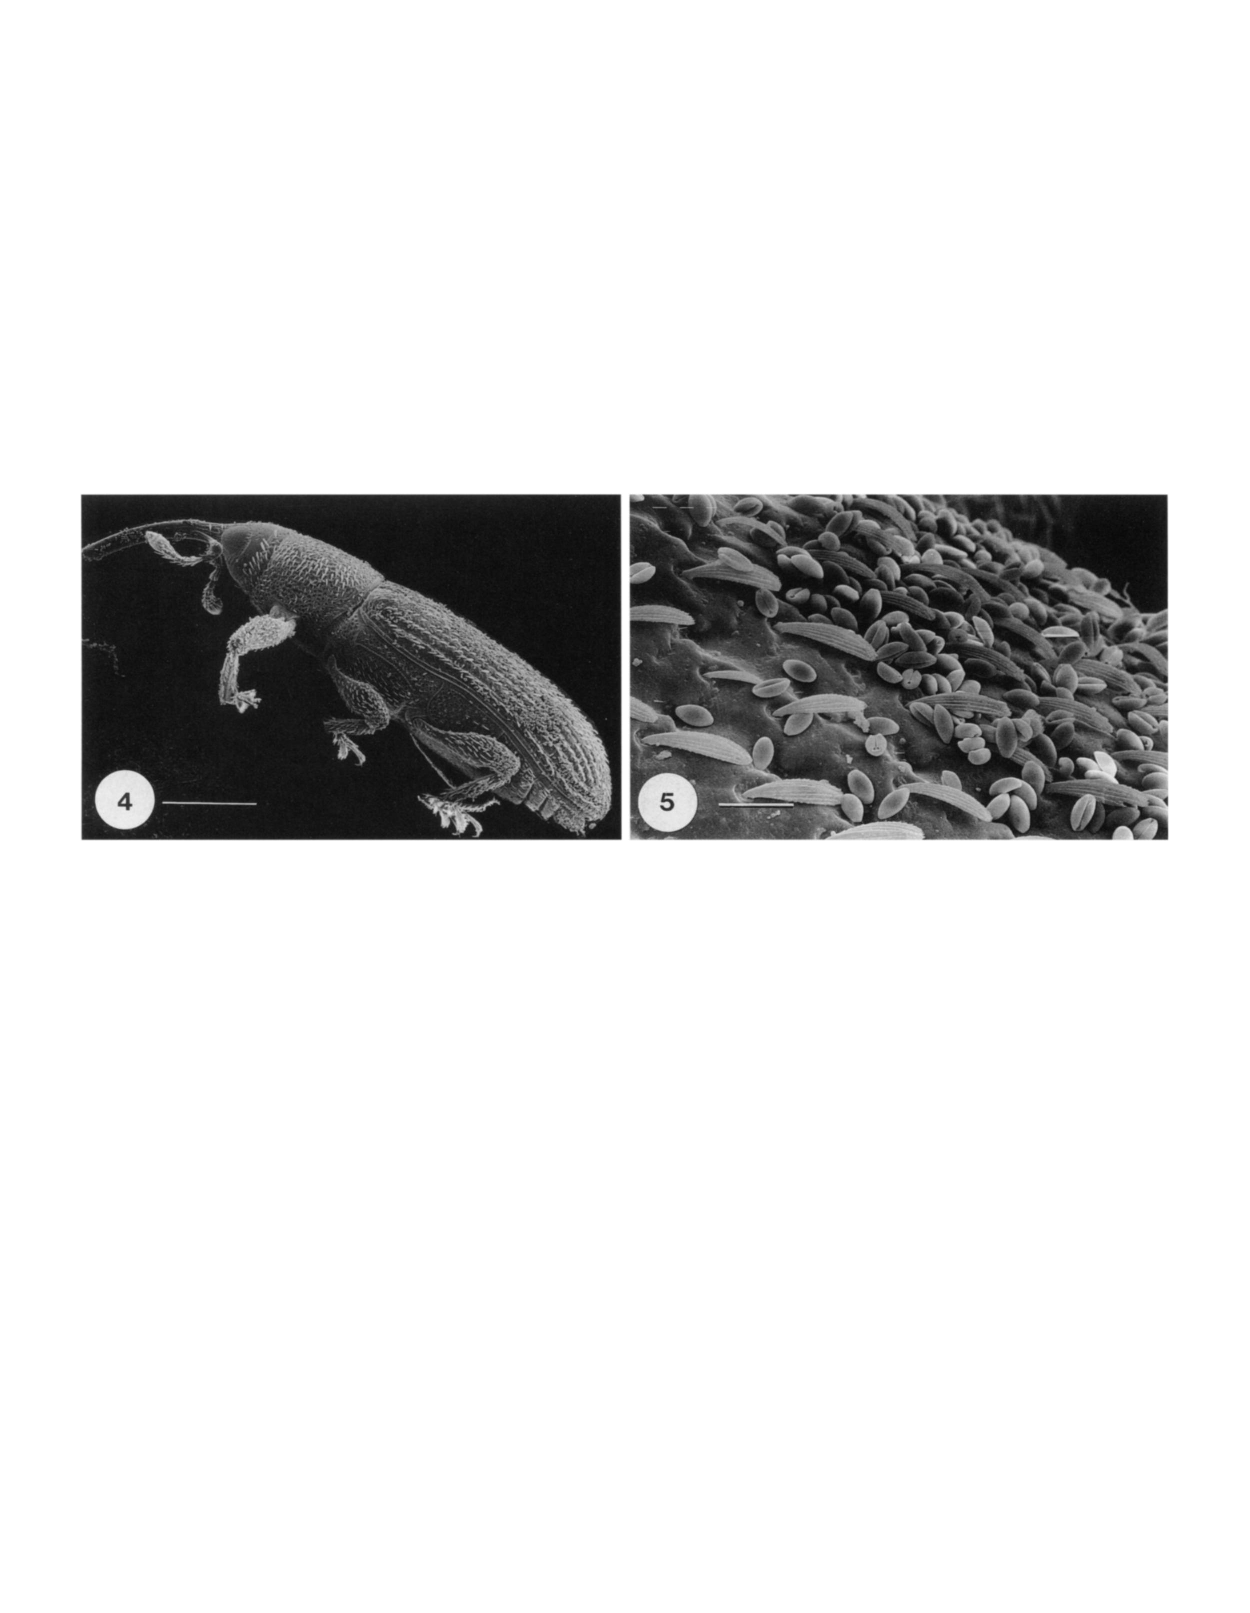
\includegraphics[width=0.81\textwidth]{figures/portheteselytra.pdf}

\includegraphics[width=0.8\textwidth]{figures/eferox.jpg}

\end{frame}

\begin{frame}{How should we compare the phylogenies of symbionts?}
\pause
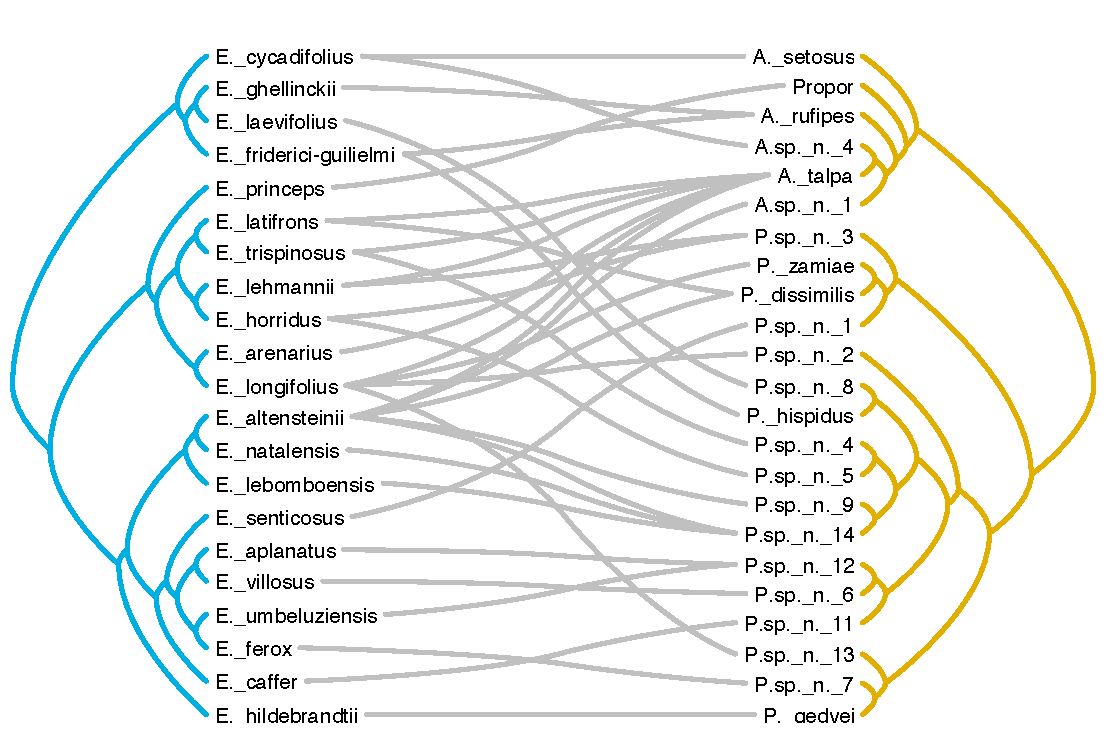
\includegraphics[width=\textwidth]{figures/tanglegram.pdf}

\end{frame}

\begin{frame}{The Cophylogeny Reconciliation Problem}

\begin{itemize}

\item What were the ancestral host--symbiont partnerships? \pause

\item Like ancestral state reconstruction, except with prior on rate matrix based on host phylogeny \pause

\item Discrepancies between host and symbiont phylogenies explained by coevolutionary events
\begin{itemize}
\item Cospeciation, duplication, host-switch, and loss
\end{itemize}

\pause

\item Also applies to gene tree--species tree reconciliation, particularly involving horizontal transfer events

\end{itemize}

\centering
\onslide<3->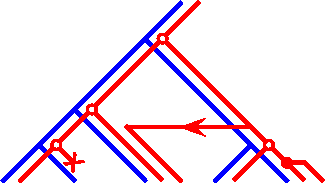
\includegraphics[width=0.5\textwidth]{beamer-pics.pdf}

%\begin{pspicture}(18,12)
%\psset{unit=0.3cm,linewidth=0.2,arrowsize=1}
%\psline[linecolor=blue](0,0)(10,10)
%\psline[linecolor=blue](4,0)(2,2)
%\psline[linecolor=blue](8,0)(4,4)
%\psline[linecolor=blue](12,0)(14,2)
%\psline[linecolor=blue](16,0)(8,8)
%\psline[linecolor=red](1,0)(11,10)
%\psline[linecolor=red,arrows=-o](17,0)(9,8)
%\psline[linecolor=red,arrows=-o](13,0)(15,2)
%\psline[linecolor=red](7,3)(14,3)
%\psline[linecolor=red,arrows=<-](10,3)(14,3)
%\psline[linecolor=red](10,0)(7,3)
%\psline[linecolor=red,arrows=-o](9,0)(5,4)
%\psline[linecolor=red,arrows=-o](4,1)(3,2)
%\rput{135}(4,1){\LARGE\textcolor{red}{\textsf{\textbf{x}}}}
%\psline[linecolor=red](18,0)(17,1)
%\psline[linecolor=red,arrows=*-](16,1)(17,1)
%\end{pspicture}

\end{frame}

\begin{frame}{Existing Work on the Cophylogeny Reconciliation Problem}

\begin{block}{Parsimony Methods}

\begin{itemize}

\item Tarzan, CoRe-PA, Jane, TreeMap, AnGST, RANGER-DTL \pause

\item Both trees must be fixed---no accommodation for uncertainty \pause

\item How to assign penalties to events or weigh numerous equally parsimonious solutions? \pause

\item Primitive consideration of node timing info \pause

\item No consideration of geographical data \pause

\end{itemize}

\end{block}

\begin{block}{Probabilistic Methods}

\begin{itemize}

\item Huelsenbeck~et~al.~(2000), Charleston~(2009), Faria~et~al.~(2013), JPrIME~DLTRS~model \pause

\item Each relies on various assumptions and simplifications

\end{itemize} 

\end{block}

\end{frame}

\section{Methods}

\begin{frame}{A Bayesian Interpretation of Cophylogeny}

\begin{equation*}
\overbrace{P\left(H,S,\R\mid D\right)}^{\mathclap{\text{probability of reconstruction}}} \onslide<2->{\propto \int_\theta \overbrace{P\left(d_H,d_S\mid H,S,\R,\theta\right)}^{\mathclap{\text{likelihood}}} \overbrace{P\left(H,S,\R,\theta\right)}^{\mathclap{\text{prior}}} \,\dif \theta}
\end{equation*}

\vspace{-12pt}

\onslide<3-4>{
\begin{block}{Likelihood}
\vspace{-12pt}
\begin{align*}
P\left(d_H,d_S\mid H,S,\R,\theta\right) &= P\left(d_H\mid H,S,\R,\theta\right)P\left(d_S\mid H,S,\R,\theta\right)\\
\onslide<4>{&= \underbrace{P\left(d_H\mid H\right)}_{\mathclap{\text{tree likelihood}}}\,\underbrace{P\left(d_S\mid S\right)}_{\mathclap{\text{tree likelihood}}}}
\end{align*}
\end{block}
}

\vspace{-96pt}

\onslide<5-6>{
\begin{block}{Prior}
\vspace{-12pt}
\begin{align*}
P\left(H,S,\R,\theta\right) &= P\left(S\mid H,\R,\theta\right)P\left(H,\R,\theta\right)\\
\onslide<6>{&= \underbrace{P\left(S\mid H,\R,\theta\right)}_{\mathclap{\text{?}}}\underbrace{P\left(H\right)P\left(\R\right)P\left(\theta\right)}_{\mathclap{\text{existing/trivial priors}}}}
\end{align*}
\end{block}
}

\vfill

$H = \text{host tree}, S = \text{symbiont tree}, \R = \text{reconciliation},$\\$\theta = \text{model parameters}, D = \left(d_H, d_S\right) = \text{sequence data}$

\end{frame}

\begin{frame}{Computing $P\left(S\mid H,\R,\theta\right)$}

\begin{itemize}

\item There are infinite histories that may yield $S$ under $H$ and $\R$
\begin{itemize}
\item Particularly confounding due to loss events
\item Probability cannot be integrated analytically
\end{itemize}
\pause

\item As a simplification, I consider only ``observable'' events \pause

\item Assume that symbiont always cospeciates with its host \pause

\item Other events independent of host and modelled as Poisson processes with independent rates \pause

\item Symbiont and host must be contemporaneous

\end{itemize}

\end{frame}

\begin{frame}{Computing $P\left(S\mid H,\R,\theta\right)$}

\centering

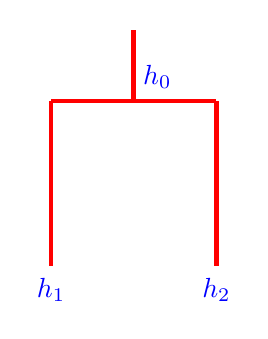
\begin{tikzpicture}[x=0.3cm, y=0.3cm, line width=0.06cm]

\draw [red] (3.5,7) -- (3.5,10);
\draw [red] (0,7) -- (7,7);
\draw [red] (0,7) -- (0,0);
\draw [red] (7,7) -- (7,0);
\node at (4.5,8) {\textcolor{blue}{$h_0$}};
\node at (0,-1) {\textcolor{blue}{$h_1$}};
\node at (7,-1) {\textcolor{blue}{$h_2$}};

\end{tikzpicture}
\pause
\begin{itemize}

\item What is the relationship of $h_0$ to $h_1$ and $h_2$ in the host tree?\pause

\item Either self, child/parent, or sister/cousin\pause

\item Permutation of two relationships yields potential scenarios

\end{itemize}

\end{frame}

\begin{frame}{Computing $P\left(S\mid H,\R,\theta\right)$: The Scenarios}

\centering

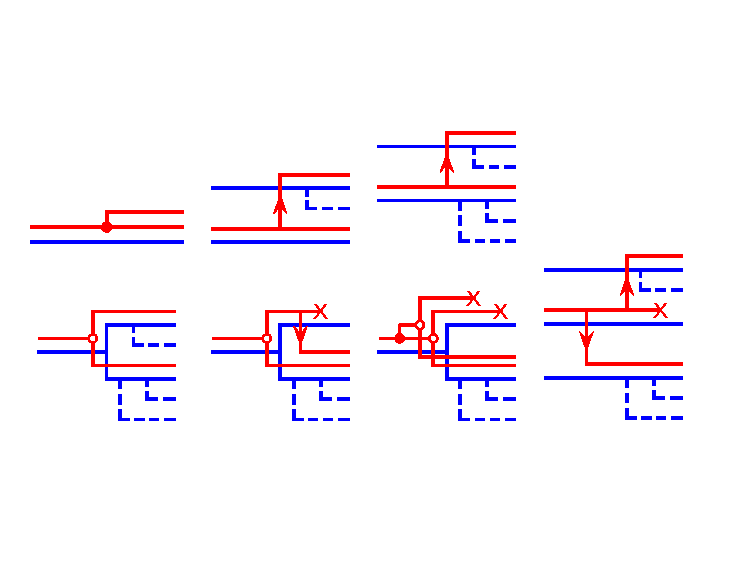
\includegraphics[width=\textwidth]{figures/scenarios.pdf}

\vspace{0.25in}\textcolor{blue}{\textbf{Host}} / \textcolor{red}{\textbf{Symbiont}}

\end{frame}

\begin{frame}{Computing $P\left(S\mid H,\R,\theta\right)$: An Example Scenario}

\centering

\begin{overprint}
\onslide<1>\centering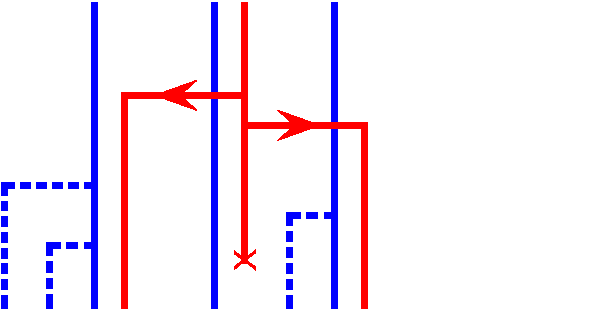
\includegraphics{figures/example_case/1.pdf}
\onslide<2>\centering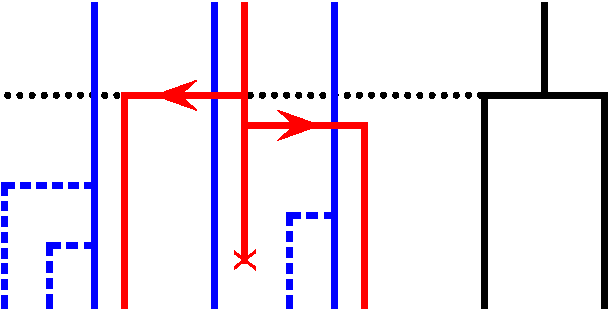
\includegraphics{figures/example_case/2.pdf}
\onslide<3>\centering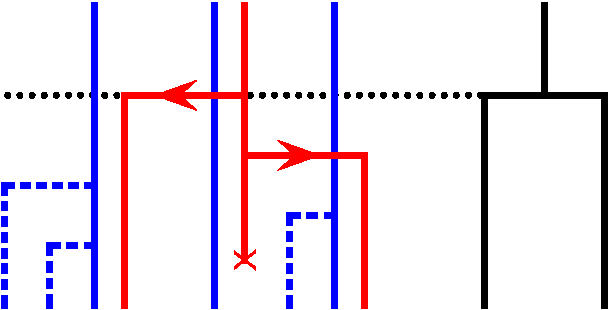
\includegraphics{figures/example_case/3.pdf}
\onslide<4>\centering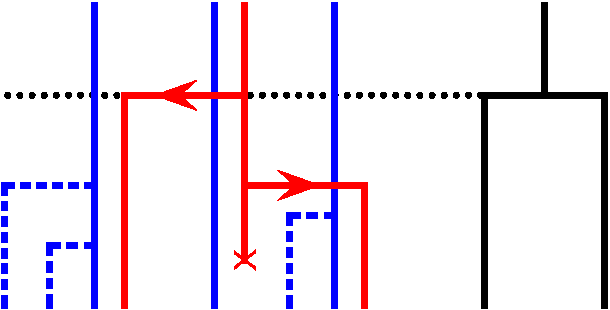
\includegraphics{figures/example_case/4.pdf}
\onslide<5>\centering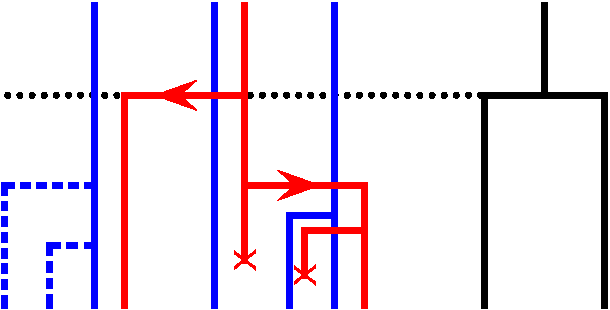
\includegraphics{figures/example_case/5.pdf}
\onslide<6>\centering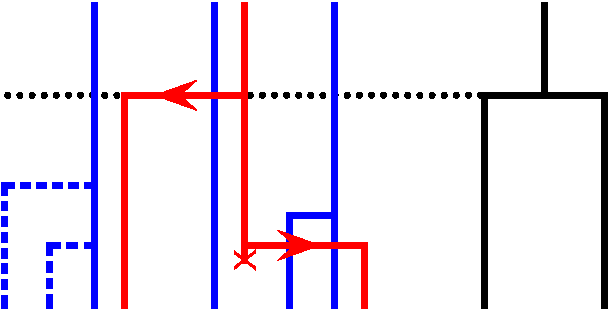
\includegraphics{figures/example_case/6.pdf}
\end{overprint}

\vspace{0.25in}\textcolor{blue}{\textbf{Host}} / \textcolor{red}{\textbf{Symbiont}}

\end{frame}

\begin{frame}{Operating on the Reconciliation}
\vfil
\begin{overprint}
\onslide<1>\centering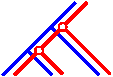
\includegraphics[page=1,width=0.5\textwidth]{figures/operator/operator-pics.pdf}
\onslide<2>\centering\includegraphics[page=2,width=0.5\textwidth]{figures/operator/operator-pics.pdf}
\onslide<3>\centering\includegraphics[page=3,width=0.5\textwidth]{figures/operator/operator-pics.pdf}
\onslide<4>\centering\includegraphics[page=4,width=0.5\textwidth]{figures/operator/operator-pics.pdf}
\end{overprint}
\vfil

%\begin{pspicture}(18,12)
%\psset{unit=0.3cm,linewidth=0.2,arrowsize=1}
%\psline[linecolor=blue](0,0)(10,10)
%\psline[linecolor=blue](4,0)(2,2)
%\psline[linecolor=blue](8,0)(4,4)
%\psline[linecolor=blue](12,0)(14,2)
%\psline[linecolor=blue](16,0)(8,8)
%\psline[linecolor=red](1,0)(11,10)
%\psline[linecolor=red,arrows=-o](17,0)(9,8)
%\psline[linecolor=red,arrows=-o](13,0)(15,2)
%\psline[linecolor=red](7,3)(14,3)
%\psline[linecolor=red,arrows=<-](10,3)(14,3)
%\psline[linecolor=red](10,0)(7,3)
%\psline[linecolor=red,arrows=-o](9,0)(5,4)
%\psline[linecolor=red,arrows=-o](4,1)(3,2)
%\rput{135}(4,1){\LARGE\textcolor{red}{\textsf{\textbf{x}}}}
%\psline[linecolor=red](18,0)(17,1)
%\psline[linecolor=red,arrows=*-](16,1)(17,1)
%\end{pspicture}

\end{frame}

\begin{frame}{Implementation Details}

\begin{itemize}

\item $\theta = (\lambda,\tau,\mu)$, rates for duplication, host-switch, and loss \pause

\item Introduce rate factor $\kappa$ represented by clock model
\begin{itemize}
\item Fix $\mu = 1$
\end{itemize}

\pause

\item Place uniform prior on $\kappa$ and gamma priors on $\lambda$ and $\tau$; \\scale operator on all \pause

\item Uniform prior on $\R$, but restricted by leaf--leaf mapping \pause

\item Implemented as plugin for BEAST1

\end{itemize}

\end{frame}

\section{Results}

\begin{frame}{Simulation Methodology}

\begin{itemize}

\item Simple simulation pipeline
\begin{enumerate}
\item Host tree generated under constant size coalescent
\item DNA simulated on host tree under JC69 model
\item Symbiont tree generated on host tree under described model (three Poisson processes)
\item DNA simulated on symbiont tree under JC69 for all extant taxa
\end{enumerate}
\pause
\item 1st simulation: 8 host taxa, all event rates 0 (identical trees)
\begin{itemize}
\item Accurate reconstruction with posterior $P\geq0.99$
\end{itemize}
\pause
\item 2nd simulation: 8 host taxa, all event rates 1.0, 8 symbionts
\begin{itemize}
\item Trees reconstructed accurately, reconciliation questionable...
\end{itemize}

\end{itemize}

\end{frame}

\begin{frame}{Results from Second Simulation}

\begin{columns}

\begin{column}{0.4\textwidth}
\null
\vspace{1in}
\begin{tabular}{r r r}

& \textbf{median} & \textbf{95\% HPD} \\\hline
$\lambda$ & $1.42$ & $[0.10,4.63]$ \\
$\tau$ & $2.48$ & $[0.20,9.18]$ \\
$\mu$ & $1.60$ & $[0.11,7.24]$

\end{tabular}

\end{column}

\begin{column}{0.6\textwidth}
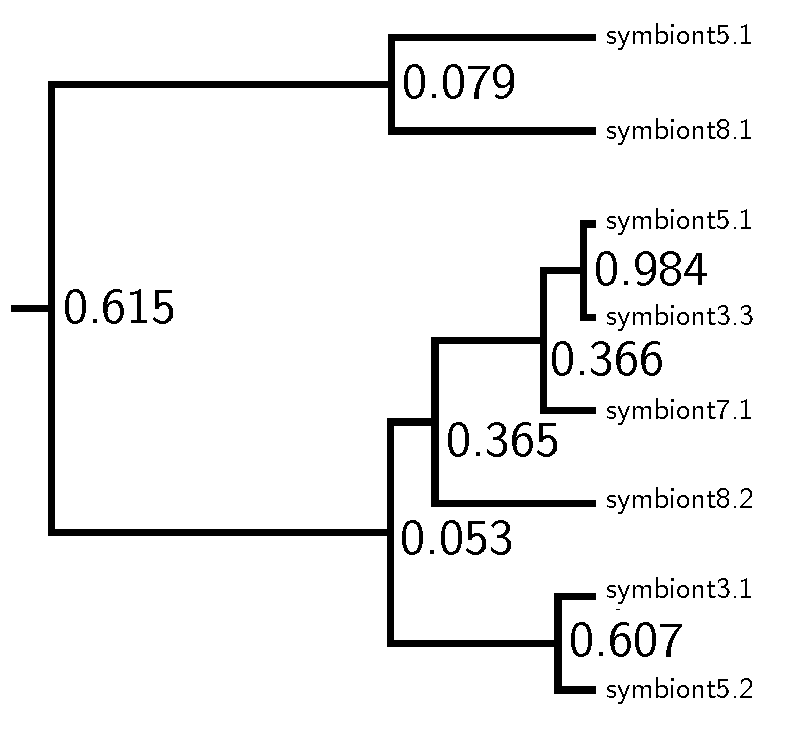
\includegraphics[width=\textwidth]{figures/sim2.pdf}
\end{column}

\end{columns}

\end{frame}

\section{Closing Remarks}

\begin{frame}{Contributions}

\begin{itemize}

\item Formulated an expression for the posterior probability of a cophylogenetic reconstruction\pause

\item Developed an algorithm to approximate the probability of a symbiont tree for a reconstruction\pause

\item Implemented the algorithm in an MCMC framework

\end{itemize}

\end{frame}

\begin{frame}{Open Questions and Problems}

\begin{block}{Detecting Cospeciation}

\begin{itemize}

\item Technically only occurs when host and symbiont speciate at the same time\pause

\item Important for identifying between some scenarios

\end{itemize}
\centering
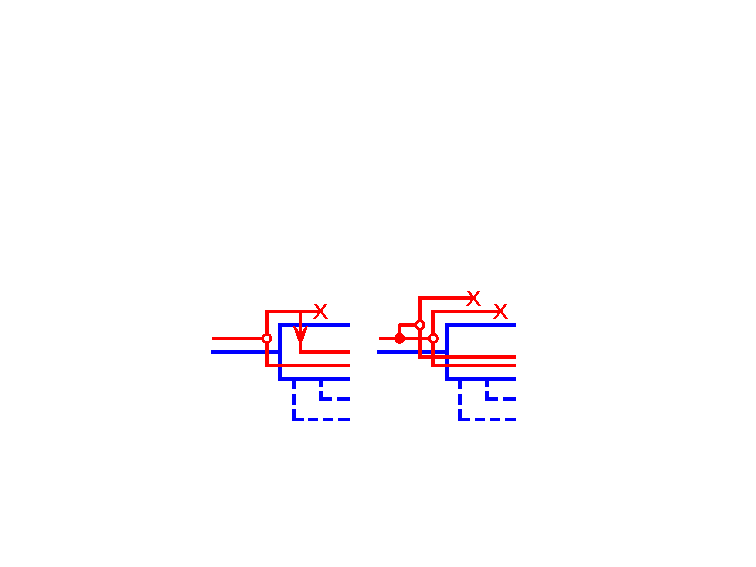
\includegraphics[width=0.9\textwidth]{figures/cospeciation-significance.pdf}

\end{block}

\end{frame}

\begin{frame}{Open Questions and Problems}

\begin{itemize}

\item Is this an appropriate approximation technique?
\begin{itemize}
\item Rigorous definition for an observable event?
\end{itemize}
\pause
\item Can we place an informative prior on the reconciliation?
\begin{itemize}
\item $P\left(H,\R,\theta\right) = P\left(\R\mid H,\theta\right)P\left(H\right)P\left(\theta\right)$
\item We have a node--node mapping $\R$, but do not know nodal relationships for one tree
\end{itemize}
\pause
\item What is the effect of the operator on mixing?
\begin{itemize}
\item Cophylogeny model substantially fragments posterior landscape---a wrong move makes the reconciliation invalid
\end{itemize}
\pause
\item How best can we evaluate the model performance via simulation studies?

\end{itemize}

\end{frame}

\begin{frame}{Open Questions and Problems}

\begin{itemize}

\item Are the event rates better predicted by the symbiont or host?
\pause
\item Model for host speciating independently of symbiont (a.k.a. failure to diverge event)?
\pause
\item Can we consider preferential host-switching in the model?
\pause
\item Can we consider geography in the model?
\begin{itemize}
\item An associated host and symbiont must be cohabiting
\end{itemize}
\pause
\item How can we visualise the reconstruction?
\begin{itemize}
\item Reconciling the trees does not recover the events
\item Several uncertainties in event timing, etc.
\end{itemize}
\pause
\item Can we test coevolutionary theories, e.g. GMTC or escape-and-radiate?

\end{itemize}

\end{frame}


\oldsection{}

\begin{frame}{Acknowledgements}

\begin{itemize}

\item My mentors, Dr.~Yi-Chieh~Jessica~Wu, Rachel~Sealfon, and Prof.~Mukul~Bansal

\item Andrew~Brownjohn, Jon~Sanders, Prof.~Ran~Libeskind-Hadas, Hayden~Metsky, and Prof.~Manolis~Kellis, for helpful discussions

\item Dr.~Susan~Offner, for inspiring me

\end{itemize}

\end{frame}

\oldsection{}

\end{document}